\documentclass{acm_proc_article-sp}

\usepackage{csquotes}
\usepackage{comment}

\usepackage{tikz}
\usetikzlibrary{shapes.geometric, arrows}

% Hyperref, uncomment if no compatibility problem.
\begin{comment}
\usepackage{hyperref}
\hypersetup{unicode}
\hypersetup{colorlinks=true}
\hypersetup{linkcolor=black}
\end{comment}

\begin{document}

\title{Secure Tropos: A Case Study on Bitmessage}
\numberofauthors{2}
\author{
% 1st. author
\alignauthor
Mukesh Jha \\ %\titlenote{Mr.~Mukesh insisted his name be first.}\\
       \affaddr{Masdar Institute}\\
       \affaddr{Masdar City}\\
       \affaddr{Abu Dhabi,UAE}\\
       \email{mjha@masdar.ac.ae}
% 2nd. author
\alignauthor
Abraham Xiao\\
  \affaddr{Masdar Institute}\\
       \affaddr{Masdar City}\\
       \affaddr{Abu Dhabi,UAE}\\
       \email{yxiao@masdar.ac.ae}
}


\maketitle
\begin{abstract}
Security is a major concern for messaging/e-mail systems. For such multi-agent systems there are various requirements such as acknowledgement, authentication etc., and security concerns like spoofing, spamming and masquerading etc. Requirement engineering and security engineering are closely inter-connected in such systems. Security modeling languages helps to analyze risks and facilitates crucial design decisions. In this paper we present an evaluation of Secure Tropos. The evaluation was carried out as a case study on Bitmessage. We analyze the concepts and terminology of Secure Tropos, its ability to address security concerns and its strengths and weaknesses in open-source software development.

\begin{comment}
. identify from the publications what are the strengths of securetropos 2. figure our how you will evaluate if these strengths are achieved in a case study 3. apply securetropos on bitmessage as a case study and produce complete set of models, trying to quantify as many things as possible (e.g., number of security requirements, goals, etc.) 4. present quantified things from (3) and discuss them 5. present the evaluation of securetropos based on (2)
\end{comment}

\end{abstract}

%\keywords{Configuration,feature models, Software Variability, Maintenance,Variability Anomalies, Bitmessage} % NOT required for Proceedings


\section{Introduction}
Secure Tropos is an extension of Tropos methodology. Tropos is a software development methodology in which concepts of agent paradigm are used. It has notions of agent, goal, task and dependency etc to model and analyze various phases of development. Secure Tropos uses those abstractions and further combines requirement engineering concepts with security engineering concepts under a unified process for development of secure software system \cite{Mouratidis06securetropos:}. Although Tropos methodology allows clear identification of dependencies between the actors, it does not capture all possible (security) constraints that might be imposed between various components \cite{Mouratidis06securetropos:}. Mouratidis et al. \cite{Mouratidis06securetropos:} have introduced various new concepts like: constraint and security constraint, secure dependency, secure entities etc. Further they have also extended the Tropos methodology by adding security modeling concepts like security reference modeling, security constraint modeling, secure entity modeling, secure capability modeling. % \mj cite the paper and tell that it is the best that i can do..
This paper will extend their work in as a case study on an open-source software which is still being actively developed and is related to security/privacy domain, i.e. Bitmessage.

%The first contribution made by this paper is the evaluation of Secure Tropos for open-source software.
%The second contribution made by this paper is the security analysis of Bitmessage.

\par
% Abraham: Actually, from my experience (lectures given by National Security Agency, China), talking about Information Security in today's % world is a joke. P.P.S., I got the degree in Information Security.

The ubiquitous form of communication in the digital world is e-mail or messaging. Since various central authorities and intermediate parties are involved between sender and receiver of the message, e-mail/messaging is inherently insecure. If \emph{any} intermediate node is compromised, the whole system becomes insecure. Moreover, various government agencies are collecting e-mail/message records and storing them in large databases for further analysis \cite{JW12}.  Under given scenario we need to have a secure communication system which doesn't depend on security state of intermediate parties. Bitmessage is a decentralized, trustless and public/private key based P2P communication protocol. It is used to send encrypted messages to another person or to many subscribers. It includes various features to overcome the problems associated with existing e-mail/message systems \cite{JW12}. Bitmessage is an open-source software which is actively being developed by different contributors. Since the prime focus of this software is security, it needs to be analyzed in light of Secure Tropos. This analysis will help in better understanding of Bitmessage security requirements and will contribute to the application level of Secure Tropos methodology.

\par %strength of secure tropos
% < include this in related work >
Dubois et al. \cite{citeulike:6509963} has extended Secure Tropos methodology for information system development. They compared Secure Tropos with the ISSRM reference model. They focused only on the early phase (early and late requirements) of the model rather than complete model. As per our best knowledge Secure Tropos has not been applied to any open-source software. Open-Source software development process is different than industrial software development process. In a typical open-source community, a group of loosely connected contributors develop separate features without actually understanding the impact of each other's module interactions. Every developer has his own understanding of security requirements for the software being developed. To remove ambiguity and provide uniform understanding, security modeling language should be applied in open-source development. We extend the Secure Tropos methodology to analyze open-source software i.e. Bitmessage, as a case study. We analyze the complete stages of Secure Tropos for Bitmessage and their relevance in open-source software development. We will use a case tool from \cite{Michalis12} to apply Secure Tropos methodology on Bitmessage. With the help of this tool we will generate a complete set of Secure Tropos methodology and analyze the models.

 %

\par
%add a label here so the codes are more "self-adaptive". (Google self-adaptive filter to find more......)
Section \ref{Sec:Related Work} presents the background and related world. Section \ref{Sec:Research Methodology} presents our research methodology.

%The most important aspect of this research is the validation of the developed solution. The Secure Tropos process allows two types of validation i.e. model validation and design validation. Further the validation rules
%

\section{Related Work}\label{Sec:Related Work}
%
%There exist a number of proposed security requirements engineering methods such as .. But Secure Tropos is the best one.. cited misuse cases, Secure-UML, UMLsec,
There are plenty security requirement engineering methods such as misuse cases, Secure-UML, UMLsec, Multilateral Security Requirements Analysis (MSRA), Secure i* etc.
These security requirement methods can be categorized as multilateral approaches (SQUARE Analysis and MSRA), Unified Modeling Language (UML)-based approaches (misuse cases, SecureUML, and UMLsec), goal-oriented approaches (Secure i*, Secure Tropos), problem frame-based approaches (abuse frames, SEPP, and SREF), risk analysis-based approaches (CORAS, and ISSRM), and CC-based approaches such as CC and SREP \cite{Husam}.



Secure Tropos is a goal-oriented security requirement engineering approach. It is an extension of Tropos methodology which is a goal oriented requirement engineering (GORE) method that supports goal-based analysis, design, and development activities. Mouratidis et al. \cite{Mouratidis06securetropos:} presented the Secure Tropos method as an extended approach of Tropos method to address the challenges of security analysis and modeling. In this method, the security requirements are considered together with other requirements and are analyzed at the early stages of system development life cycle. It supports a number of security-related concepts such as secure goal, security constraint, security dependency and security task etc.

In this section we discuss various papers related to Security requirement engineering and Secure Tropos.
\par
``Tropos is an information system development methodology, tailored to describe both the organizational environment of a system and the system and the system itself", as illustrated by Castro et al. \cite{Jaelson01}. And on the basis of Tropos, Mouratidis extended it to Secure Tropos by adding security concerns, which have raised more attention in the development process of Information Systems recently.
In \cite{Jaelson01}, the researchers first extended concepts defined in Tropos, which are security constraint, secure dependency, as well as secure entities. For secure entities, they could represent either a secure goal, secure task or secure source. After the renewal of related concepts, they were used in respecting secure modelling, an example is security constraint modelling. When the modelling part is finished, there are 3 more steps in Secure Tropos process to be carried out. Firstly, system requirements are to be identified. Secondly, a design meeting not only system functional requirements but security requirements is to be identified. Thirdly, a validation of the developed solution is to be done.
\par
Rehman and Mustafa did a broad research on software design level security vulnerabilities\cite{Rehman:2009:RSD:1640162.1640171}. They analyzed specific software design tasks, vulnerabilities as well as mitigation mechanisms based on other people's findings. This paper serves as an indicator helping us choose more related papers. % Really a junk paper, comment this paragraph if you feel it sucks.
\par
Aronk et al.\cite{Aaronk10} pointed out in his paper that in paper \cite{Massacci2005445}, the researchers just utilized a goal-modeling approach to requirements compliance, not having being able to represent traceability information. So they put forward a set of methods to capture as well as refractor links between security requirements and legal texts (referring to both legislation and regulations). Their first step is to build three categories---Actors, Data Objects and Actions. These categories are used to classify terminology mapping between software requirements and legal texts. The second step is to ``identify" the mapping produced in the first step, namely to produce a different set of modified requirements. As can be inferred, the third step uses output of the second one, and elaborates on them. Results are called disambiguated requirements that software engineers can understand. The final step merely builds links between the ``elaborated" requirements and legal texts. Aronk's team used a health record system named iTrust as a case study.

\par
Nadzeya et al.\cite{Nadzeya08}did research on application of requirement specification transformation. They experimented methods in building semi-structured specifications from natural language described ones. More specifically, they used a light-weight method (Cerno)\cite{Nadzeya06} during requirements elicitation phase to extract them , hoping that their findings could better support Secure Tropos methodology. They used the semantic annotation environment, namely Cerno, to parse specifications in natural language. Their steps are as follows. First is to parse senario description and structure it according to pre-defined document grammar rules. Then the document anotation is done using the scenario definition vocabulary. A further step is to markup more complex relationships with the help of domain- and input-driven patterns. The final step is to assign semantic roles. It's obvious that roles are varied depending on their positions in the statement. Their work has helped us better understand the Secure Tropos framework. % Abraham: Add your conclusion of their work here. Just one line.



\section{Research Methodology}\label{Sec:Research Methodology}
We are using case study as a research methodology. This type of study facilitates holistic analysis, understanding and exploration of systems. Case study researchers like Stake, Halen and Yin suggest that this method of research excels at bringing an understanding of a complex issues or object and helps to extend already known ideas through previous research. Yin suggested that this methodology can be effectively used for both quantitative and qualitative research. In this case study we are extending and applying Secure Tropos on Bitmessage.

\par
It is very important to have a clear design plan for the case study. This provides an effective method to perform specific research. There are various ways a case study can be performed such as interviews, journals etc. Case studies can be divided into holistic or embedded studies \cite{37844699}. In this work, we have adopted a holistic (single unit of analysis). Anderson \cite{37844699} defined holistic case study as an approach to examine the case as one unit.
\par
The design plan of our case study is shown in the flow chart figure \ref{fig:Design Plan}. The research work in this paper first starts with understanding Secure Tropos methodology and Bitmessage. This is followed by identifying the research objectives. Then, the research questions which are one by one explored in this work are presented. Bitmessage is used as an unit of analysis in this work. Based on Secure Tropos methodology various security reference models of Bitmessage are created. This is followed by the analysis of the models and its evaluation.

\tikzstyle{startstop} = [rectangle, rounded corners, minimum width=3cm, minimum height=1cm,text centered, draw=black]

\tikzstyle{io} = [trapezium, trapezium left angle=70, trapezium right angle=110, minimum width=3cm, minimum height=1cm, text centered, text width=2cm, inner sep=2pt, draw=black, inner sep=2pt]
\tikzstyle{process} = [rectangle, minimum width=3cm, minimum height=1cm, text centered, text width=3cm, draw=black]
%\tikzstyle{decision} = [diamond, minimum width=3cm, minimum height=1cm, text centered, draw=black]

\tikzstyle{arrow} = [thick,->,>=stealth]

\begin{figure}
\begin{tikzpicture}[node distance=2cm]

\node (start) [startstop] {Start};

\node (pro1) [process, below of=start] {Research Objective};
\draw [arrow] (start) -- (pro1);
\node (in1) [io, right = 1.5cm, right of=pro1] {Evaluation of Secure Tropos};
\draw [arrow] (in1) -- (pro1);

\node (pro2) [process, below of=pro1] {Research Questions};
\draw [arrow] (pro1) -- (pro2);
\node (in1) [io, right = 1.5cm, right of=pro2] {Secure Tropos applications};
\draw [arrow] (in1) -- (pro2);

\node (pro3) [process, below of=pro2] {Unit of analysis};
\draw [arrow] (pro2) -- (pro3);
\node (in1) [trapezium, trapezium left angle=70, trapezium right angle=110,minimum height=10pt,  text centered, text width=2cm, draw=black, inner sep=0pt, right = 1.5cm, right of=pro3] {Bitmessage};
\draw [arrow] (in1) -- (pro3);

%\node (pro4) [process, below of=pro3] {Data Collection};
%\draw [arrow] (pro3) -- (pro4);
%\node (in1) [io, right = 1.5cm, right of=pro4] {Resarch papers on Secure Tropos};
%\draw [arrow] (in1) -- (pro4);

\node (pro5) [process, below of=pro3] {Model Creation};
\draw [arrow] (pro3) -- (pro5);
\node (in1) [io, right = 1.5cm, right of=pro5] {Create different security reference models};
\draw [arrow] (in1) -- (pro5);

\node (pro6) [process, below of=pro5] {Model Analysis};
\draw [arrow] (pro5) -- (pro6);
\node (in1) [io, right = 1.5cm, right of=pro6] {Analyze Model and link to research questions};
\draw [arrow] (in1) -- (pro6);

\node (pro7) [process, below of=pro6] {Evaluation};
\draw [arrow] (pro6) -- (pro7);
\node (in1) [trapezium, trapezium left angle=70, trapezium right angle=110,minimum height=10pt,  text centered, text width=2cm, draw=black, inner sep=2pt, right = 1.5cm, right of=pro7] {Evaluation Criteria};
\draw [arrow] (in1) -- (pro7);

\node (end) [startstop, below of=pro7] {End};
\draw [arrow] (pro7) -- (end);
\end{tikzpicture}
\caption{Case Study Design Plan Flow-Chart}\label{fig:Design Plan}
\end{figure}
\par
The research objective of this case study is to evaluate the application of Secure Tropos on open-source software by applying this methodology to analyze Bitmessage (as a case study). We analyze the Secure Tropos through the complete set of security reference models which are generated for Bitmessage.
\par
The research questions of this case study can be listed as:
\begin{enumerate}
\item What are the security requirement, security constraints and major security scenarios for Bitmessage?
\item What is the relevance of individual security reference model generated by Secure Tropos?
\item What are the security scenarios that needs critical understanding or are being missed?
\item How can we enhance Secure Tropos to handle security modeling for open-source software?
\end{enumerate}

In order to evaluate the application of Secure Tropos on open-source software, we have characterized the security requirements of Bitmessage and analyzed if the models generated by Secure Tropos is able to capture them.
%The software development process is distinctly different in case of open-source.

\begin{comment}
\subsection{Analyze Bitmessage}
We will analyze the architecture and features of Bitmessage. Bitmessage is actively being developed by an open-source community. This software is concerned with security and privacy of e-mail/messaging. Hence it is very crucial for this software to undergo security analysis. We apply Secure Tropos methodology to understand its security requirements and possible attack scenarios.
\end{comment}

\subsection{Generate Secure Tropos Security models}
Secure Tropos considers basic Tropos concepts and adds security concepts like constraint, secure plan, secure resource etc. It consists following modeling activities:
\begin{enumerate}
\item Security reference modeling: This involves concepts like security features, protection objectives, security mechanisms and the threats that have a negative contribution towards the security features of the system. This reference diagram can be used as a reference point throughout the development process.

\item  Security constraint modeling: This involves the concept of security constraints imposed to actors and the system. This allows developers to analyze relationships between a security constraint and its context or the relationship between different security constraints.

\item Secure entities modeling. This involves the analysis of the secure entities of the system.

\item Secure capability modeling: This involves the identification of the secure capabilities of different actors, which in turn, guarantees the fulfillment of security constraint.
\end{enumerate}

\subsection{Analyze Models}
Various models generated using Secure Tropos needs to be analyzed to quantify if they are  able to capture the security requirement of Bitmessage. The quantified security requirements of Bitmessage and the capability of models to capture them will evaluate the Secure Tropos model. This will further help in evaluating the application of Secure Tropos on open-source software.

\subsection{Result}
In this section we discuss the results obtained by applying Secure-Tropos method on Bitmessage as case study. We analyzed each stage as required by the secure torpos method. We present each step diagram and it's corresponding analysis.

\begin{enumerate}
\item Early Requirement: For each project to be successful it is very important to understand it's existing organizational settings. In this phase we analyzed the organizational model of Bitmessage, different actors associated with it, their dependencies and security constraint imposed on them.  

\begin{itemize}
\item Sender : Can send messages, encrypt message, ask for public-key, validate address etc.
\item Receiver : Can receive message, decrypt message, send acknowledgement etc.
\item Peer : broadcast the message.
\end{itemize}

Bitmessage is a peer-to-peer message protocol, the main actors involved in this protocol are Sender, Receiver and a set of intermediate peers between them. Since peer could be an actor or a group of actors it makes more sense to model it as a set. Since peer has no other function than to broadcast the massage, it plays trivial role. The main focus of early stage it to capture the organizational settings which is clearly depicted  in \ref{fig:fig2}.
 
\begin{figure}[ht!]\label{fig:fig2}
\centering
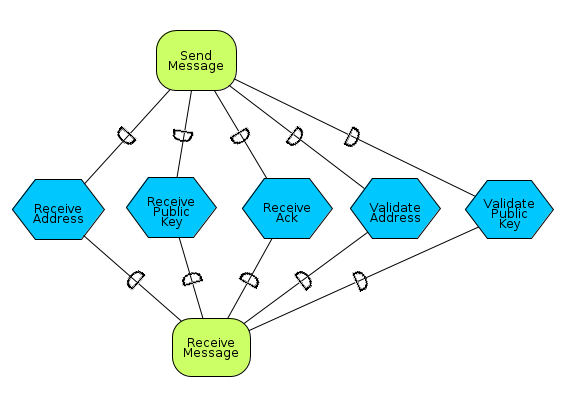
\includegraphics[width=90mm]{Early-Requirements.png}
\caption{Early Requirement}
\label{f1.1}
\end{figure}

\item Enhanced Goal With Constraints Modeling: In this phase, we captured the enhanced goal of the system in details and inherent problems, security constraints and attack scenarios. As shown in figure \ref{f1.1} we modeled the complete system, actors, their behaviors, functions and constraints among them. 

\begin{figure}[ht!]
\centering
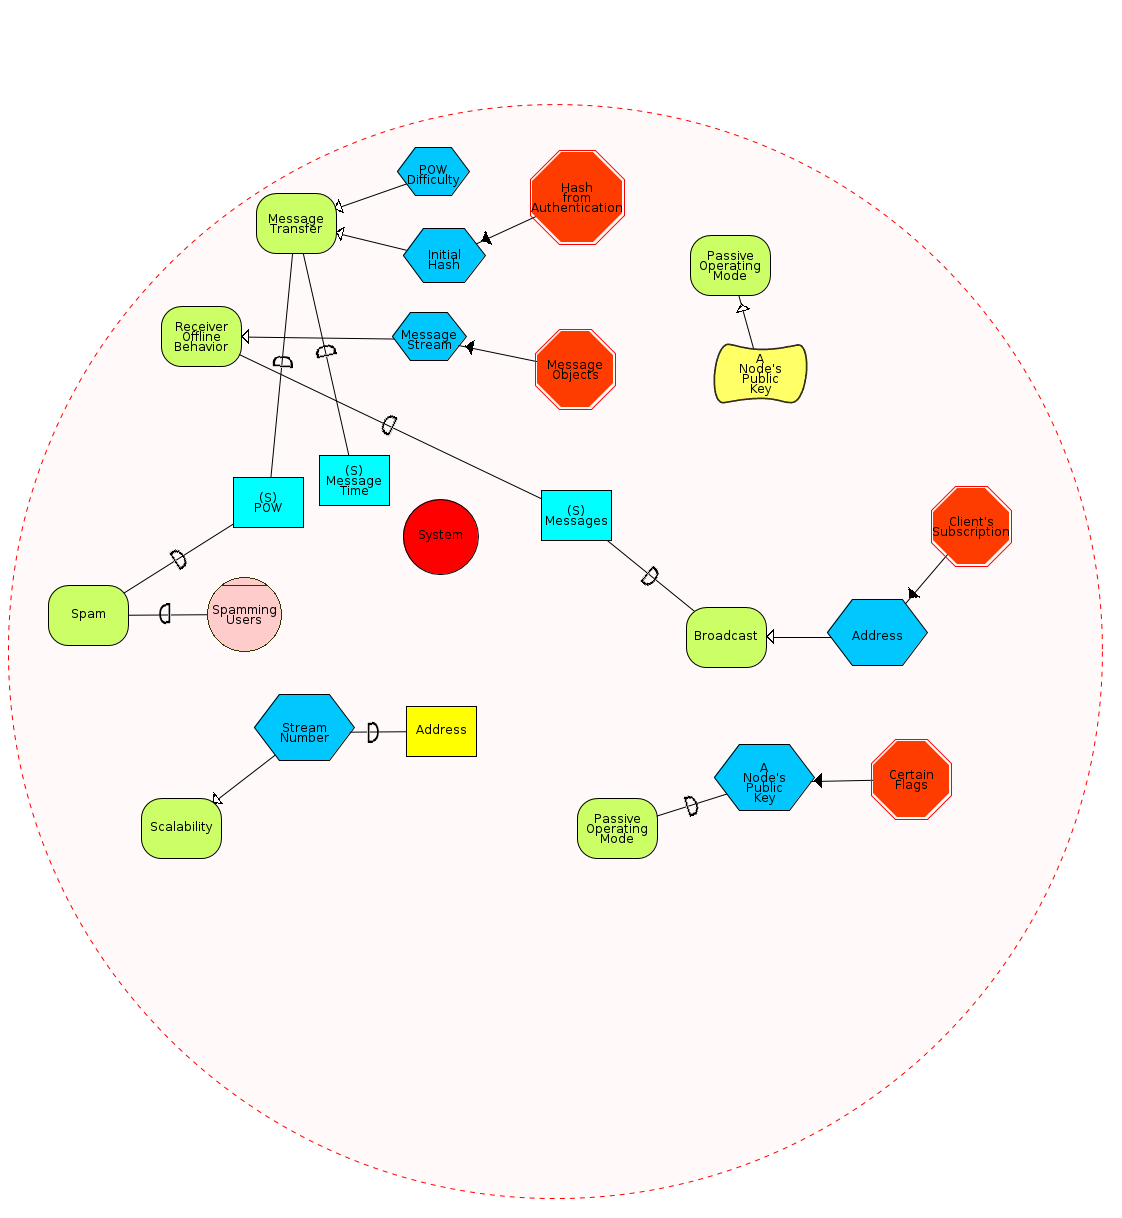
\includegraphics[width=90mm]{Enhanced-Goal-With-Constraints.png}
\caption{Enhanced Goal With Constraints}
\label{f1.2}
\end{figure}

\item Secure Entities : In this stage, we modeled the high-level organization of the complete system and represent  any secure goals/tasks/resources of the system. A secure goal represents the strategic interests of an
actor with respect to security. In case of Bitmessage, the secure goal of sender is to securely encrypt the message and broadcast it to all peers. Secure goals help to achieve possible security constraints that are imposed to an actor. A secure resource can be defined as an informational entity that is related to the security of the multiagent system. In case of Bitmessage the encrypted message can be defined as a very important resource. The Bitmessage is focused on securing the message transferred between sender and receiver based on private-public key encryption scheme.  

\begin{figure}[ht!]
\centering
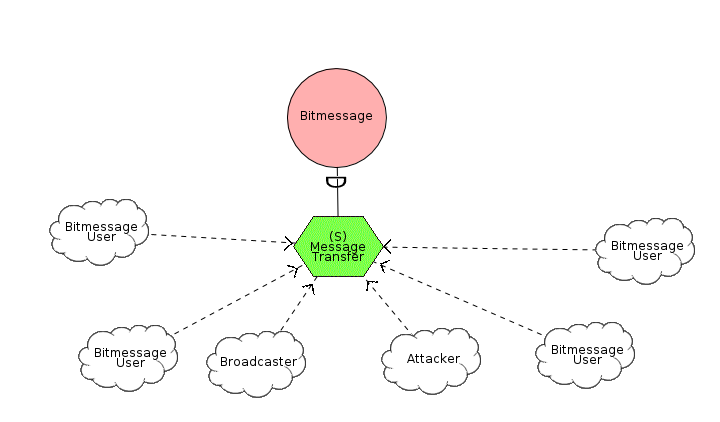
\includegraphics[width=90mm]{Secure-Entities.png}
\caption{Secure-Entities}
\label{f1.3}
\end{figure}

\end{enumerate}

\subsection{Evaluation}
In this section, we evaluate the results of applying Secure-Tropos on Bitmessage. Overall, during the analysis of Bitmessage, we discovered Secure-Tropos is able to capture most of security scenarios. We analyzed the major security threats imposed on Bitmessage system. We discovered specific vulnerabilities and threats:
\begin{itemize}
\item This system should have feature of login before the datafile is read. Any attacker with physical possession of device can read the messages by simply running the software.

\item For same pass-key used by any actors for generating address, private-public key are also same. It is a valid contention that different users might end up using same pass-key. 

\item The security requirement that it should prevent user from modifying forwarded message or detect the modified forwarded messages is not being clearly applied.

\item The system should prevent spamming. It is a serious issue in any mailing system. Bitmessage implements Proof-of-Work concept to discourage spamming. This is a measure to discourage attacker but not a full-proof method.
\end{itemize}
 
We found serious flaws in Bitmessage by using Secure-Tropos and analyzing its security requirements. Bitmessage fails to secure it's resource on host device. It should provide login facility and symmetric encryption for data files on device as well. Since it is associated with security of messages, this requirement is not considered by the application.  
 
\subsection{Conclusion}
Secure-Tropos is useful too for security analysis of open-source software. Before starting an open-source project, it is imperative for the community to analyze the security aspect of project. We discovered that Secure-Tropos is not capturing the concept of sets. For a group of actors can be grouped together as per their similar roles. In case of Bitmessage, all the intermediate actors between sender and receiver can be grouped as a set of peers. There can be hierarchy among actors, and combination of actors might result in enhanced roles or constraints. To enable Secure-Tropos with the power of set and hierarchy it needs to include these concepts.  

\bibliographystyle{abbrv}
\bibliography{sigproc}
\end{document}
